\chapter{Codec Timing}

Figure \ref{graph:codec-speeds} shows a comparison of encode and decode times across varying quality factors for each of the conduit image implementations. Due to limited testing equipment and the length of the tests CPU load could not be kept uniform - these results give only an approximation of the timing involved. Section XXX gives a more accurate overview of time spent encoding and decoding for the 3-bit scaling conduit image class.

\begin{figure}[tbph]
  \begin{center}
    
\subfigure{
\begin{tikzpicture}
    \begin{axis}[grid=major,xlabel=JPEG Quality Factor,ylabel=Encoding time (ms),
    height=5cm,width=10cm,legend style={legend pos=outer north east}]
    
    \addplot
        table[x=QF,y=e_Sc3] {gfx/encoding_time.data};
    
    \addplot
        table[x=QF,y=e_Sc4] {gfx/encoding_time.data};
        
    \addplot
        table[x=QF,y=e_Haar] {gfx/encoding_time.data};
        
    \legend{Scaled3,Scaled4,Haar}
    
    \end{axis}
\end{tikzpicture}
}
\subfigure{
\begin{tikzpicture}
    \begin{axis}[grid=major,xlabel=JPEG Quality Factor,ylabel=Decoding time (ms),
    height=5cm,width=10cm,legend style={legend pos=outer north east}]
    
    \addplot
        table[x=QF,y=d_Sc3] {gfx/encoding_time.data};
    
    \addplot
        table[x=QF,y=d_Sc4] {gfx/encoding_time.data};
        
    \addplot
        table[x=QF,y=d_Haar] {gfx/encoding_time.data};
        
    \legend{Scaled3,Scaled4,Haar}
    
    \end{axis}
\end{tikzpicture}
}

    \caption{Per image encode and decode times for each of the three conduit image implementations, for varying JPEG quality factors.}
    \label{graph:codec-speeds}
  \end{center}
\end{figure}

\begin{figure}[tbph]
    \begin{center}
\begin{tikzpicture}
\begin{axis}[xlabel=Time (seconds), ylabel=Frequency,
grid=major,const plot, ymin=0, enlargelimits=false,
width=12cm, height=5cm, legend style={area legend}]

    \addplot[fill=blue, fill opacity=0.5] table[x=t,y=Text] {gfx/async_text_hist.data};
    
    \addplot[fill=red, fill opacity=0.5] table[x=t,y=Text_c] {gfx/async_text_hist.data};
    
    \addplot+[sharp plot,blue, mark=no marker] coordinates
        {(6.403,0) (6.403,56)};
        
    \addplot+[sharp plot,red, mark=no marker] coordinates
        {(3.463,0) (3.463,56)};
    
    \legend{Cache off,Cache on}
\end{axis}
\end{tikzpicture}

\begin{tikzpicture}
\begin{axis}[xlabel=Time (seconds), ylabel=Frequency,
grid=major,const plot, ymin=0, enlargelimits=false,
width=12cm, height=5cm, legend style={area legend}]
    
    \addplot[fill=blue, fill opacity=0.5] table[x=t,y=Images] {gfx/async_image_hist.data};
    
    \addplot[fill=red, fill opacity=0.5] table[x=t,y=Images_c] {gfx/async_image_hist.data};
    
    \addplot+[sharp plot,blue, mark=no marker] coordinates
        {(19.169,0) (19.169,130)};

    \addplot+[sharp plot,red, mark=no marker] coordinates
        {(4.067,0) (4.067,130)};
    
    \legend{Cache off,Cache on}
    
\end{axis}
\end{tikzpicture}
    \caption{Histogram of 400 page loading times for newsfeeds containing 15 encrypted messages (top) and 15 encrypted images (bottom).}
    \label{graph:hist}
  \end{center}
\end{figure}


\begin{figure}[tbph]
    \begin{center}
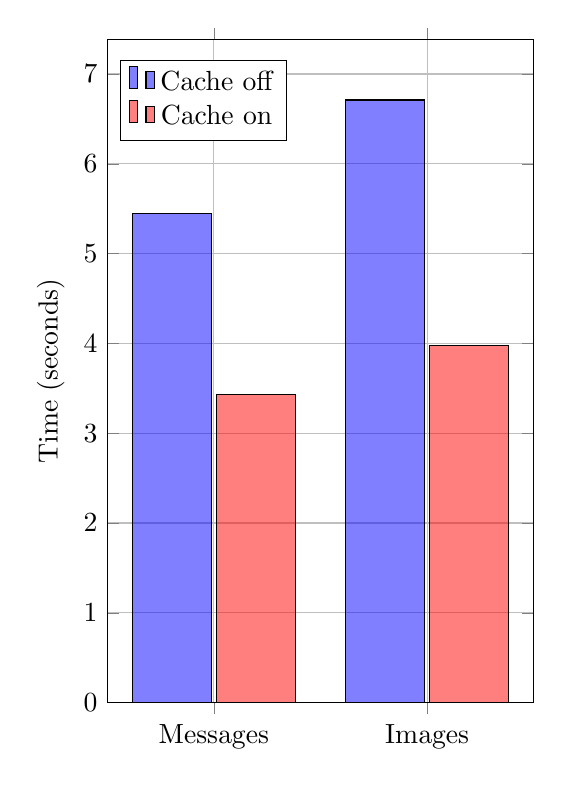
\begin{tikzpicture}
\begin{axis}[grid=major,ybar, 
    symbolic x coords={Messages,Images},
    xtick=data,ylabel=Time (seconds), width=7cm, height=10cm,
    legend style={legend pos=north west, area legend},
    bar width=1cm,enlarge x limits=0.5,ymin=0]
        \addplot[fill=blue, fill opacity=0.5] coordinates { (Messages,5.4457) (Images,6.7105) };
        \addplot[fill=red, fill opacity=0.5] coordinates { (Messages,3.4306) (Images,3.9765) };
        \legend{Cache off, Cache on}
\end{axis}
\end{tikzpicture}
    \caption{Average time before first encrypted item loads.}
    \label{graph:time-first}
  \end{center}
\end{figure}

\begin{figure}
    \begin{center}
        \begin{tikzpicture}
        \begin{axis}[grid=major,ycomb,
        ylabel=Time (ms), 
        width=12cm, height=5cm,
        bar width=0.3cm, ymin=0, xmin=2, xmax=15, enlarge x limits=0.04]
            \addplot[blue] table[x=Item,y=Text] {gfx/async.data};
        \end{axis}
        \end{tikzpicture}
        \begin{tikzpicture}
        \begin{axis}[grid=major,ycomb,
        ylabel=Time (ms), xlabel=Message,
        width=12cm, height=5cm,
        bar width=0.3cm, ymin=0, xmin=2, xmax=15, enlarge x limits=0.04]
            \addplot[red] table[x=Item,y=Text_c] {gfx/async.data};
        \end{axis}
        \end{tikzpicture}
    \caption{Average time interval between successive message loads, with caching turned off and on (top and bottom respectively).}
    \label{graph:txt-rest}
    \end{center}
\end{figure}

\begin{figure}[tbph]
\begin{center}
    
\begin{tikzpicture}
\begin{axis}[grid=major,ycomb,
ylabel=Time (ms), 
width=12cm, height=5cm,
bar width=0.3cm, ymin=0, xmin=2, xmax=15, enlarge x limits=0.04]
    \addplot[blue] table[x=Item,y=Image] {gfx/async.data};
\end{axis}
\end{tikzpicture}

\begin{tikzpicture}
\begin{axis}[grid=major,ycomb,
ylabel=Time (ms),xlabel=Image,
width=12cm, height=5cm,
bar width=0.3cm, ymin=0, xmin=2, xmax=15, enlarge x limits=0.04]
    \addplot[red,] table[x=Item,y=Image_c] {gfx/async.data};
\end{axis}
\end{tikzpicture}

\caption{Average time interval between successive image loads, with caching turned off and on (top and bottom respectively).}
\label{graph:img-rest}
\end{center}
\end{figure}